\documentclass[a4paper,11pt,oneside]{report}
\usepackage[pdftex]{graphicx}
\usepackage[utf8x]{inputenc}
\usepackage[spanish]{babel}
\usepackage{fancyhdr}
\usepackage[Bjornstrup]{fncychap}
\usepackage{tabularx}
\usepackage{hyperref}
\usepackage{eurosym}
\usepackage{longtable}
\usepackage[table]{xcolor}
\usepackage{verbatim}
% \usepackage[usenames,dvipsnames]{color}
% \usepackage{colortbl}
% \usepackage[caption=false]{subfig}
% \usepackage{float}
% \usepackage{pdflscape}

\setlength{\headheight}{25pt}
\setlength{\parskip}{6pt}

% Margenes 1cm mas pequennos
% \addtolength{\oddsidemargin}{-1cm}
% \addtolength{\evensidemargin}{-1cm}
% \addtolength{\textwidth}{2cm}
% \addtolength{\voffset}{-1cm}
% \addtolength{\textheight}{2cm}

\lhead{
\includegraphics[height=20pt]{logo-umbrella.png}}
\chead{}
\rhead{\nouppercase{\leftmark}}

\hypersetup{
colorlinks,
citecolor=black,
filecolor=black,
linkcolor=black,
urlcolor=black
}

 % La que hay que liar para que las cabeceras de los capitulos
 % no tiren media pagina a la basura...

\makeatletter
\def\@makechapterhead#1{{
\parindent \z@ \raggedright \normalfont
\ifnum \c@secnumdepth >\m@ne
	\if@mainmatter
		\DOCH
	\fi
\fi
\interlinepenalty\@M
\if@mainmatter
	\DOTI{#1}
\else
	\DOTIS{#1}
\fi
}}

\def\@makeschapterhead#1{{
\parindent \z@ \raggedright
\normalfont
\interlinepenalty\@M
\DOTIS{#1}
}}
\makeatother

\begin{document}

\renewcommand\listtablename{Índice de tablas}
\renewcommand\tablename{Tabla}

\pagestyle{plain}

%%%% Title Page %%%%%

\pagenumbering{alph}

\begin{titlepage}
\begin{center}

% Logo

\includegraphics[width=0.6\textwidth]{logo-umbrella.png}\\[4cm]

% Title
{\huge \textbf{La Conquista del Mundo}}\\[0.5cm]
{\huge {Memoria del proyecto}}\\[4cm]

% Authors
\begin{minipage}{0.5\textwidth}
\large
\hspace{1cm}\textbf{\emph{Director de proyecto}}\\
Ricardo Ruedas García\\
\end{minipage}

\begin{minipage}{0.5\textwidth}
\large
\hspace{1cm}\textbf{\emph{Equipo de desarrollo}}\\
Jorge Colao Adán\\
Ángel Durán Izquierdo\\
Antonio Gómez Poblete\\
Daniel León Romero\\
Antonio Martín Menor de Santos\\
Laura Núñez Villa\\
\end{minipage}\\[2cm]

{\Large \today}
\end{center}
\end{titlepage}

%%%% end Title Page %%%%%

\clearpage
\pagenumbering{arabic}
\setcounter{page}{2}

\tableofcontents
\addcontentsline{toc}{chapter}{\contentsname}
% \listoffigures
% \listoftables

\clearpage

\pagestyle{fancy}

\chapter{Introducción}

\section{Descripción del juego}

\textit{La Conquista del Mundo} es un juego de estrategia por turnos que es
jugado sobre un tablero que representa el mapa del mundo. Este mapa está
dividido en 42 territorios.

Cada jugador comienza con un territorio y, por turnos, podrá realizar distintas
acciones como comprar nuevas unidades o territorios, o invadir territorios
enemigos. Todas estas acciones van dirigidas a alcanzar el objetivo del juego:
conquistar el mundo.

\section{Sistema distribuido}

La aplicación constituye un sistema distribuido. Los alumnos de la asignatura
formarán un total de cinco grupos. De éstos, uno de ellos se encargará del
desarrollo del servidor. El resto de grupos, entre los que se incluye éste,
realizarán independientemente clientes para este sistema.

Las comunicaciones entre las distintas aplicaciones se realizarán haciendo uso
del \textit{middleware} de comunicaciones RMI de Java. Para ello, se ha escrito
una interfaz común de clases para transmitir los datos entre los clientes y
el servidor.

\section{Visión general del documento}

% TODO

\chapter{Arquitectura}

La aplicación sigue una variación de la arquitectura de tres capas. Las capas
de presentación y dominio permanecen inalteradas. Sin embargo, esta aplicación
no necesita de almacenamiento externo, sino que se obtiene esta información
directamente del servidor. Por ese motivo, la capa de persistencia ha sido
sustituida por una capa de comunicaciones.

\begin{figure}[h]
\caption{Visión general de la arquitectura}
\centering
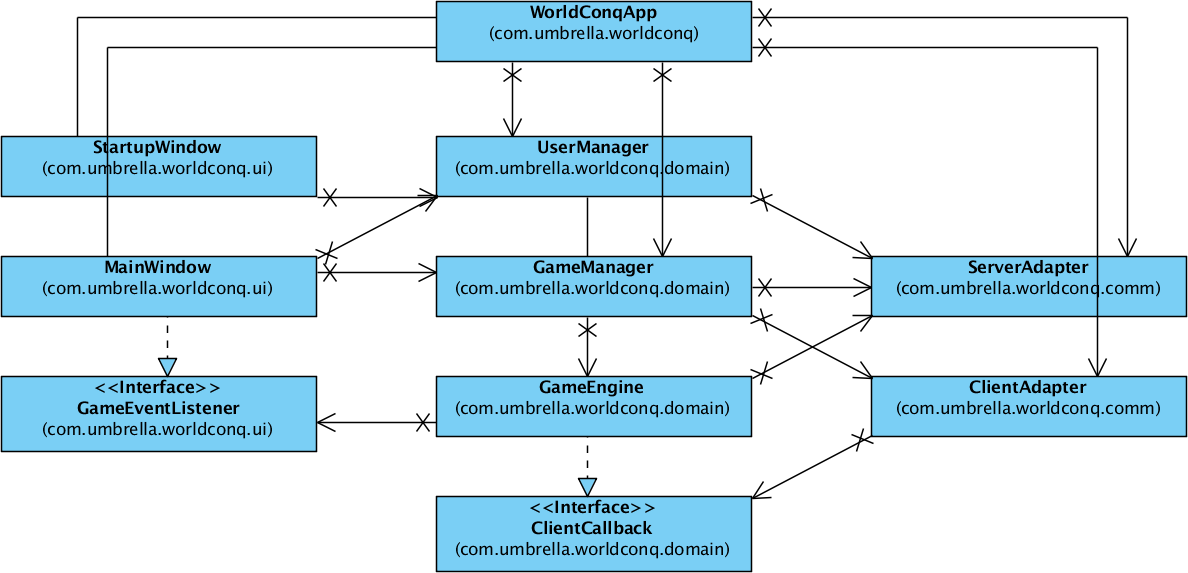
\includegraphics[scale=0.4]{img/ch02arch-overview.png}
\end{figure}

La visibilidad entre clases va de manera jerárquica, de manera que las clases
de presentación conocen a las de dominio, y las de dominio a las de
comunicaciones, pero no al revés. Para los casos en los que es necesario un
flujo de información en sentido contrario, se han creado interfaces para
desacoplar en la medida de los posible las capas inferiores.

La clase \texttt{WorldConqApp} es la única clase que no pertenece a ninguna de
las capas. Su función es la de ser el punto de entrada de la aplicación,
encargada de crear la estructura de clases, sus relaciones, y configurarlas a
partir de los parámetros de entrada.

\section{Capa de comunicaciones}

Esta capa contiene las clases \texttt{ServerAdapter} y \texttt{ClientAdapter}.
Ambas clases sirven de pasarela para los datos que fluyen entre el servidor y la
capa de dominio.

Estas clases incluyen una pequeña lógica de control. En el caso de la clase
\texttt{ServerAdapter}, ésta debe ser configurada con los datos del servidor
para así poder crear el \textit{proxy} a la interfaz remota. La ausencia de
esta configuración generará una excepción.

La clase \texttt{ClientAdapter} en cambio escucha todas las peticiones que
realiza el servidor sobre el cliente. Esta clase filtra estas peticiones de
acuerdo al juego activo en ese momento, descartando aquellas que no concuerden.

\section{Capa de dominio}

Esta capa está dividida en tres clases que se corresponden con los tres módulos
funcionales de la aplicación: gestión de usuarios, gestión de partidas, y motor
de juego.

La clase \texttt{UserManager} es la encargada de crear nuevas cuentas en la
aplicación y de mantener la información de la sesión activa. A esta clase
acceden el resto de clases para obtener la información sobre el jugador. De
manera análoga, la clase \texttt{GameManager} gestiona el listado, creación y
carga de partidas.

\begin{figure}[h]
\caption{Modelos de datos}
\centering
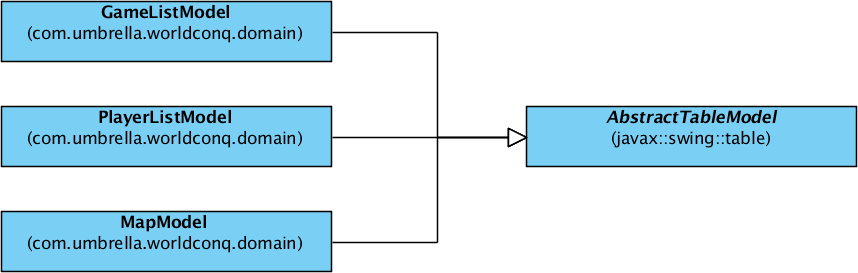
\includegraphics[scale=0.4]{img/ch02arch-models.png}
\end{figure}

Los datos de las partidas disponibles en el servidor son almacenados en objetos
de tipo \texttt{GameListModel}. Esta clase, y otras que se describen a
continuación, heredan de la clase \texttt{AbstractTableModel}. Esta clase
abstracta forma parte del \textit{framework} que proporciona Swing para
implementar el patrón arquitectónico Model-Vista-Controlador.

Hacer uso de este \textit{framework} significa que los accesos que hacen las
vistas a los modelos están definidos de antemano por una serie de interfaces.
Esto permite asociar clases disponibles en Swing con clases implementadas por el
equipo de trabajo de forma transparente.

En último lugar está el motor de juego, la clase \texttt{GameEngine}. Esta
clase se crea al comenzar a jugar a una partida e implementa toda la lógica de
dominio de una partida. Los datos con los que trabaja están almacenados en las
clases \texttt{PlayerListModel} y \texttt{MapModel}, los cuales heredan de la
clase \texttt{AbstractTableModel}, nombrada anteriormente.

\section{Capa de presentación}

En esta capa se encuentra la clase \texttt{StartupWindow}. Esta clase
representa a la primera ventana que se muestra. En ella, el usuario puede
registrar un nuevo usuario en el sistema y acceder con él.

Una vez accedido, se muestra la ventana principal, representada por la clase
\texttt{MainWindow}. Dentro de esta ventana existen dos modos de ejecución: el
modo de sala de espera y el modo partida.

\begin{figure}[h]
\caption{Vistas de datos}
\centering
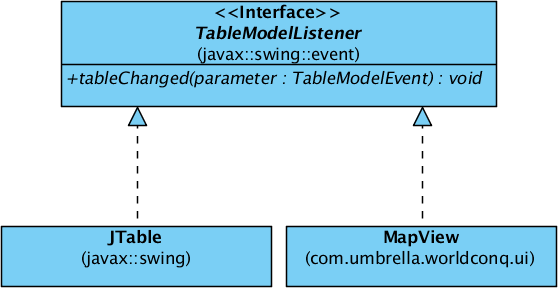
\includegraphics[scale=0.4]{img/ch02arch-views.png}
\end{figure}

En el modo de sala de espera, el usuario puede ver las partidas disponibles o
crear otras nuevas. Una vez se decida a cual jugar, la aplicación pasa a modo
partida.

La interfaz del modo partida se compone principalmente del mapa de juego. Junto
a él existen otro paneles informativos con los jugadores en la partida o una
lista con los últimos eventos.

Tanto las listas de partida como el mapa de juego implementan la interfaz
\texttt{TableModelListener}. Esto permite que estas clases puedan ser añadidas
como observadores de los cambios que sucedan en los modelos de datos.

\chapter{Desarrollo}

En este capítulo se hará un seguimiento del desarrollo completo del proyecto,
organizado por casos de uso. Para cada caso de uso, se comenzará hablando sobre
las decisiones de diseño tomadas. Un siguiente apartado tratará sobre cualquier
aspecto relevante de la implementación. Por último se mostrará un informe de
pruebas.

La documentación de este capítulo no sustituye al proyecto realizado con Visual
Paradigm, sino que destaca los aspecto más importantes para su mejor
comprensión.

\subsection{Registrarse}

\begin{figure}[ht]
\centering
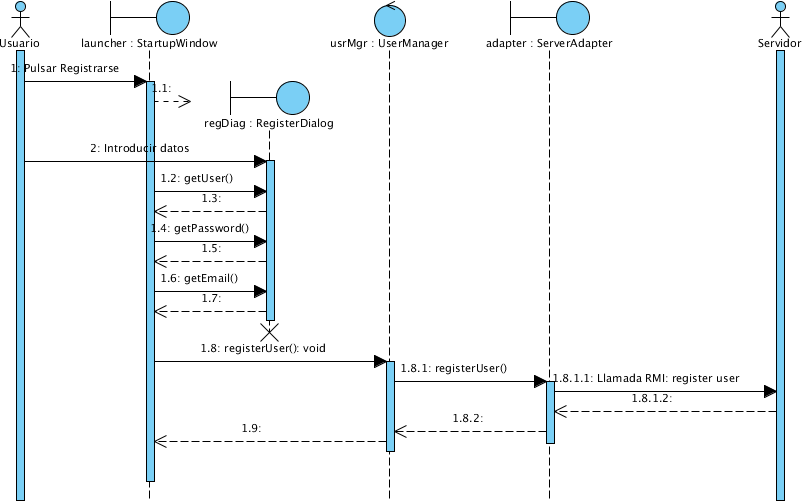
\includegraphics[scale=0.6]{img/ch03devel-register.png}
\caption{Diagrama de secuencia de ``Registrarse''}
\end{figure}

Cuando el usuario pulse el botón ``Registrarse'', se mostrará el diálogo de
registro \texttt{RegisterDialog}. Este diálogo se ejecutará de manera modal,
por lo que bloqueará el flujo de ejecución en la aplicación principal hasta que
el usuario lo complete.

A continuación, la aplicación llamará a la función correspodiente en el gestor
de usuarios para llevar a cabo el registro. Éste a su vez realizará la llamada
RMI a través del \texttt{ServerAdapter}.

Este caso de uso no provoca cambios en el estado interno del gestor de usuarios.

\subsection{Iniciar sesión}

\begin{figure}[ht]
\centering
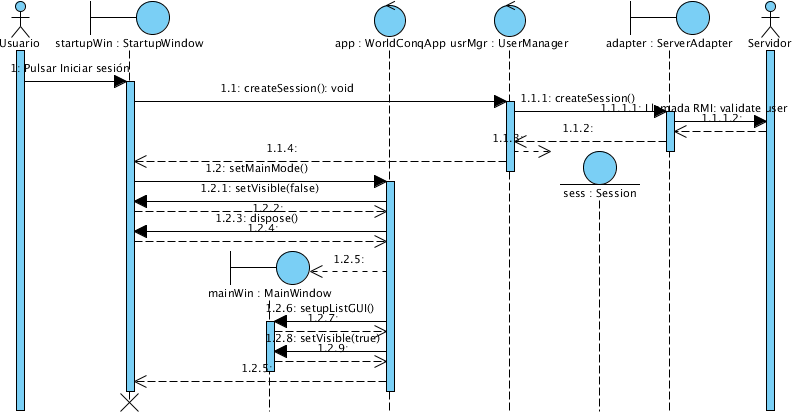
\includegraphics[scale=0.6]{img/ch03devel-login.png}
\caption{Diagrama de secuencia de ``Iniciar sesión''}
\end{figure}

Una vez que el usuario haya introducido sus credenciales, la ventana
\texttt{StartupWindow} pedirá al gestor de usuarios que inicie una nueva
sesión. El gestor de usuarios realizará la llamada RMI a través del
\texttt{ServerAdapter}.

Si los datos son correctos, el servidor devolverá un identificador de sesión.
Con este identificador y el propio nombre de usuario, el gestor de usuarios
creará un nuevo objeto de tipo \texttt{Session}.

A continuación, la ventana \texttt{StartupWindow} pedirá a la clase
\texttt{WorldConqApp} el cambio al modo principal. Al realizar este cambio, se
ocultará la ventana de inicio y se creará la nueva ventana principal
\texttt{Mainwindow}.

\subsection{Cerrar sesión}

\begin{figure}[ht]
\centering
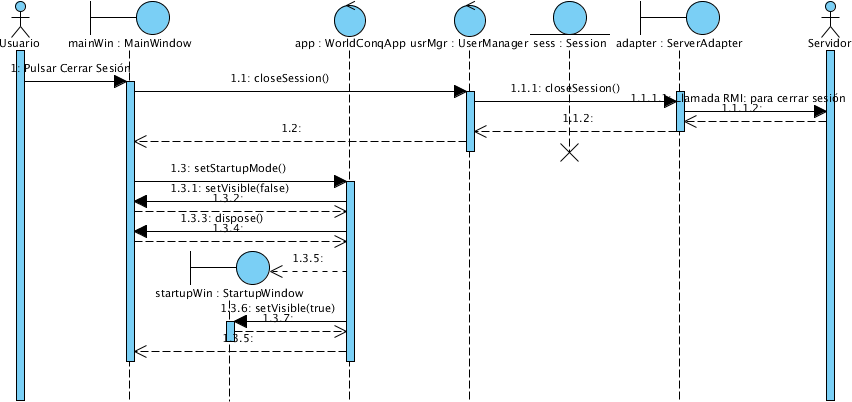
\includegraphics[scale=0.6]{img/ch03devel-logout.png}
\caption{Diagrama de secuencia de ``Cerrar sesión''}
\end{figure}

Estando en la ventana principal, el usuario puede decidir cerrar sesión en
cualquier momento. Este evento genera una llamada al gestor de usuarios. El
gestor de usuarios comunica al servidor que el usuario quiere cerrar la sesión.
Así mismo, destruirá la sesión que había hasta ahora.

A continuación se solicita a la clase \texttt{WorldConqApp} que vuelva a la
ventana de inicio realizando el paso inverso al detallado en la sección
anterior.

\subsection{Actualizar la lista de partidas}

\begin{figure}[ht]
\centering
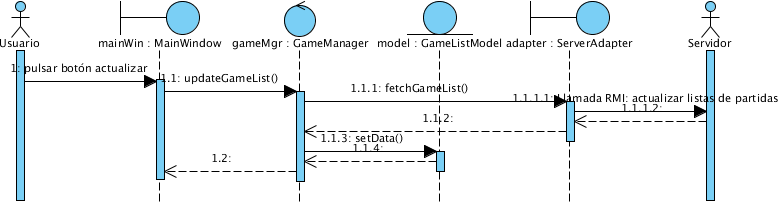
\includegraphics[scale=0.6]{img/ch03devel-listgames.png}
\caption{Diagrama de secuencia de ``Actualizar la lista de partidas''}
\end{figure}

Estando en la ventana principal, el usuario puede realizar una serie de
acciones. Una de ellas puede ser actualizar la lista de partidas mostrada. Ante
esta acción, el gestor de partidas solicitará una nueva lista al servidor a
través del \texttt{ServerAdapter}.

La lista recibida desde el servidor debe ser filtrada y organizada en dos
sublistas: una con partidas abiertas para unirse, y otra con partidas en las
que esté participando el usuario y estén activas en este momento.

Una vez seleccionadas las partidas, éstas son asignadas a dos objetos de tipo
\texttt{GameListModel}. Puesto que las vistas, dos \texttt{JTable}, han sido
configuradas como observadores de estos modelos, su actualización es llevada a
cabo por el \textit{framework} automáticamente.

\subsection{Crear una partida}

\begin{figure}[ht]
\centering
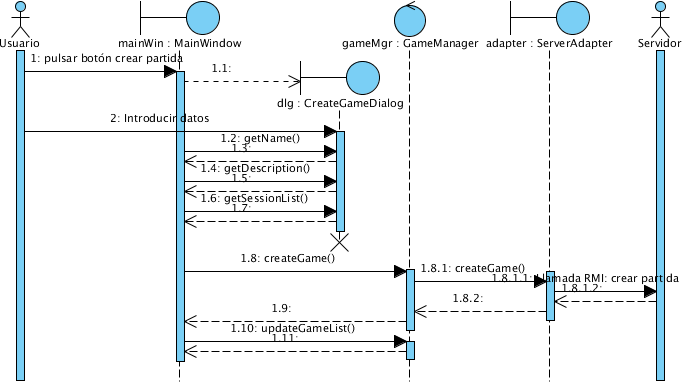
\includegraphics[scale=0.6]{img/ch03devel-creategame.png}
\caption{Diagrama de secuencia de ``Crear una partida''}
\end{figure}

Cuando el usuario seleccione la opción de crear una nueva partida, se le
mostrará una ventana diálogo donde podrá seleccionar los parámetros de esta
nueva partida.

Con estos datos, la ventana principal solicitará al gestor de partidas la
creación de una nueva partida. Si no ocurre ninguna excepción, se realizará una
llamada al caso de uso anterior, actualizar lista de partidas, para que se
actualicen los modelos de datos, y por tanto la interfaz de usuario.

\section{Unirse a una partida}

\begin{figure}[ht]
\centering
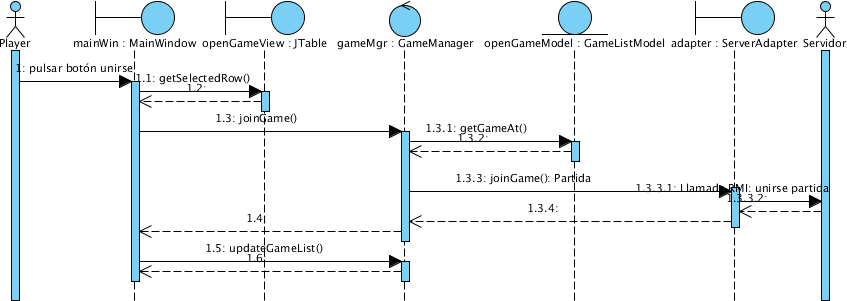
\includegraphics[scale=0.6]{img/ch03devel-joingame.png}
\caption{Diagrama de secuencia de ``Unirse a una partida''}
\end{figure}

Al seleccionar una partida listada en la vista de partidas disponibles, se
activará el botón para unirse a ella. Al pulsar este botón, la ventana
principal obtendrá el índice de la partida seleccionada y llamará a la función
correspondiente del gestor de partidas.

Utilizando el índice proporcionado desde la interfaz, el gestor de partidas
obtendrá el objeto \texttt{GameInfo} que representa a la partida seleccionada.
A continuación pedirá al \texttt{ServerAdapter} que efectúe la unión a la
partida en el servidor.

Al igual que ocurría en el caso de uso anterior, se llamará a la funcionalidad
de actualizar la lista de partidas para que la interfaz muestre los cambios
producidos.

\section{Conectarse a una partida}

\begin{figure}[ht]
\centering
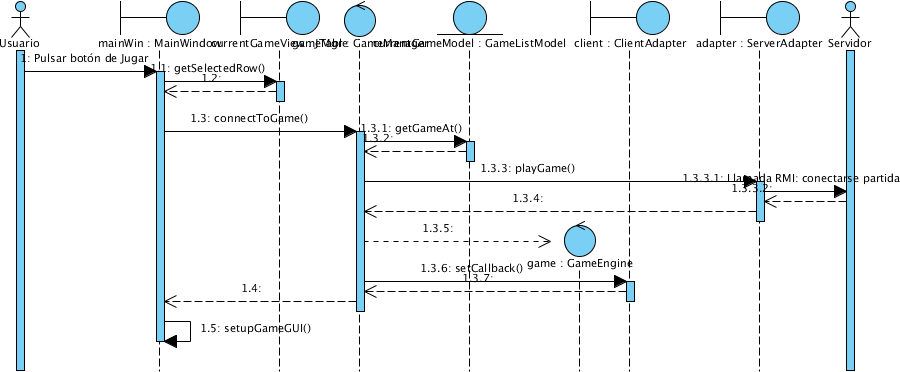
\includegraphics[scale=0.6]{img/ch03devel-playgame.png}
\caption{Diagrama de secuencia de ``Conectarse a una partida''}
\end{figure}

Si se selecciona una partida a la que el usuario ya se haya unido previamente,
podrá entonces ejecutar la acción de jugar en esa partida. Al igual que en el
caso anterior, la ventana principal obtendrá el índice de la partida a partir
de la vista.

El gestor de partidas realizará la petición al servidor de comenzar a jugar en
la partida seleccionada. Es entonces cuando el gestor de partidas creará un
objeto de tipo \texttt{GameEngine} a partir de los datos devueltos por el
servidor.

Esta clase está encargada de toda la lógica del juego, e implementa todos los
casos de uso relacionados con el módulo de juego. Dentro de ella se crean los
dos modelos de datos básicos en cada partida: \texttt{MapModel} y
\texttt{PlayerListModel}.

La clase \texttt{MapModel} almacena la información de los 42 territorios que
tiene una partida. Los datos de cada territorio son accesibles al completo a
través de la función \texttt{getTerritoryAt}. Sin embargo, si se accede a través
de la función \texttt{getValueAt} definida por el \textit{framework}, los datos
devueltos son filtrados de acuerdo a las reglas del juego. Esto es así porque
las vistas usarán esta última función, y de esta forma la vista no necesita
realizar ninguna lógica de control sobre los datos. La clase
\texttt{PlayerListModel} funciona de manera análoga con la lista de jugadores.

El motor del juego también debe responder a las peticiones que llegan del
servidor. Para ello se ha creado la interfaz \texttt{ClientCallback}, la cual
implementa. Una vez creado el objeto de tipo \texttt{GameEngine}, éste es
pasado al \texttt{ClientAdapter} para que redirija las peticiones que lleguen
del servidor.

Finalmente, cuando dominio ha terminado de preparar los datos, la ventana
principal carga la nueva interfaz de partida. Ésta está compuesta por tres
vistas: \texttt{MapView}, \texttt{PlayerView}, y \texttt{TerritoryInfoView}.

Todas estas vistas implementan la interfaz \texttt{TableModelListener}, a la
vez que se registran como observadores de los modelos correspondientes. La
vista \texttt{TerritoryInfoView} muestra información sobre el territorio
seleccionado en el mapa. Por ese motivo, esta clase también debe registrarse
como observador del modelo de selección de la clase \texttt{MapView}.


\chapter{Procesos de gestión}

En este capítulo se muestra una descripción no técnica de los procesos que han
influido en el desarrollo de la práctica.

\section{Actividades}

Para el desarrollo de esta práctica, se han desempeñado las siguientes
actividades.

\subsection*{Especificación de requisitos}

Realizada durante las primeras dos semanas, esta actividad consitió en una
lectura detallada del enunciado de la práctica para extraer las funcionalidades
que la aplicación debía tener.

Del desarrollo de esta actividad se obtuvo el documento \textit{UC 01-002.01
Especificación de requisitos software}, que describe de una manera más
detallada y directa el alcance de la aplicación. Además se generó el diagrama
de modelos de casos de uso, que muestra esquemáticamente todos los requisitos
funcionales de la aplicación.

\subsection*{Análisis y diseño}

Partiendo de la especificación de requisitos, los analistas-diseñadores
realizarán en esta actividad una serie de acciones que definirán el diseño de
la arquitectura de la aplicación y las relaciones existentes entre las clases
de la misma.

Resultado de esta actividad habrá como mínimo un \textit{diagrama de secuencia}
por cada caso de uso. En estos diagramas se muestra en un nivel de detalle medio
el flujo de mensajes entre clases para la consecución de un determinado caso de
uso.

Con el conocimiento obtenido del análisis de cada caso de uso se irán creando de
manera incremental los \textit{diagramas de clases}. El resultado son tres
diagramas por cada capa arquitectónica, y un cuarto diagrama de clases que
muestra las relaciones entre las clases más importantes a alto nivel.

\subsection*{Implementación}

Esta actividad materializa el diseño realizado en la actividad anterior. El
resultado será una nueva versión de la aplicación con la funcionalidad
correspondiente.

La brevedad de este apartado no refleja el tiempo invertido en esta actividad
con respecto al resto de actividades. Esta actividad no se limita a programar,
sino que a veces es necesario resolver problemas técnicos que pueden sergir
durante la programación.

\subsection*{Pruebas}

Con esta actividad se busca la validación y verificación de los componentes de
la aplicación, a nivel tanto individual como de conjunto. Las pruebas
se han realizado usando el \textit{framework} de pruebas \textit{JUnit} en
combinación con el analizador de covertura \textit{EclEmma}.

De esta actividad se ha obtenido una extensa batería de pruebas que prueban el
comportamiento a nivel de integración de toda la capa de dominio.

Por su excesiva complejidad, se decidió no probar programáticamente la capa de
presentación de la aplicación. En su lugar, se crearían guiones de pruebas
exploratorias.

\subsection*{Documentación}

Actividad de cierre del proyecto, dentro de esta actividad se incluye la
redacción del presente documento, los informes de las pruebas realizadas en la
actividad anterior, o el manual de usuario de la aplicación.

En el entregable final, presentado en un DVD, se incluirán todos los artefactos
generados por las actividades aquí explicadas.

\section{Planificación}

De la planificación mostrada en el documento \textit{UC 01-001.02 Plan de
gestión de proyecto software} se podía decir en su día que era muy optimista. A
día de hoy, se puede decir que aquella planificación era extremadamente
optimista.

Únicamente las dos o tres primeras semanas se cumplieron hasta cierto grado.
Sin embargo la incertidumbre de no estar aún disponible la interfaz de
comunicaciones ralentizó el proceso de analisis y diseño hasta pararlo por
completo.

Se tomó la decisión de no continuar con el desarrolló hasta que la interfaz no
estuviera definida para no realizar trabajo que tuviera que ser desechado más
adelante por no ajustarse a la especificación.

Aún con todo, retrospectivamente se pueden apreciar distintas fases en el
desarrollo que en mayor o menor medida conciden con las del proceso unificado.

\subsection{Fase de inicio}

\textit{Del 6 de octubre al 31 de octubre}

Durante estas aproximadamente tres semanas y media, las actividades realizadas
se ajustaron a la planificación expuesta en el plan de proyecto. En este
período se redactaron el plan gestión de proyecto software y la especificación
de requisitos software.

En los últimos días, se inicio con las actividades de análisis y diseño. Se
llegaron a cubrir los primeros casos de uso, todos relacionados con la gestión
de usuarios.

\subsection{Fase de elaboración}

\textit{Del 1 de noviembre al 25 de diciembre}

Esta fase estuvo marcada por la falta de una interfaz de comunicaciones
definida y estable. Se necesitaba avanzar en el proceso de diseño, pero a la
hora de definir las clases, sus atributos, y los argumentos usados en los
métodos, siempre surgía la duda de qué datos se usarían.

Esto no significa que el equipo estuviera totalmente parado, pero sí que el
rendimiento estaba muy por debajo del posible, y del deseado. Se realizaron los
diagramas de secuencia de hasta el sexto caso de uso, casi todos los
relacionados con la gestión de partida, intentando usar los valores que se
creían más adecuados. Así mismo, se empezó con la implementación del módulo de
gestión de usuarios. Estas funciones eran relativamente sencillas y era poco
probable que el trabajo hecho fuera a resultar incorrecto al tener la interfaz
definitiva.

El día 22 de diciembre tuvo lugar la reunión de jefes de grupo de la que surgió
la primera versión estable de la interfaz de comunicaciones, y que
posteriormente sólo sufriría cambios menores. En los días siguientes a esa
fecha, y con una idea mucho más clara de la arquitectura de la aplicación de la
que se tenía en octubre, se repasaron todos los diagramas realizados hasta la
fecha. Este hito dio por concluida la fase de elaboración.

\subsection{Fase de construcción}

\textit{Del 26 de diciembre al 27 de febrero}

El primer paso de esta fase fue reescribir el código para que se ajustara a los
cambios realizados en diseño, lo cual no supuso un gran esfuerzo.

Durante el mes de enero, el rendimiento fue también bajo debido a ser el
período de exámenes. En este mes se realizaron dos elementos importantes en
diseño y en implementación.

Por un lado, se empezó la implementación del caso de uso ``Conectarse a una
partida''. Este caso de uso es la base para todos los que vendrían a
continuación. En él se obtienen los datos de una partida, se configura dominio
creando el motor de juego, y se carga la interfaz de partida, la cual incluye
el mapa. Es una actividad bastante extensa que no estaría terminada hasta el 5
de febrero.

Paralelamente, los analista-diseñadores estuvieron trabajando en el caso de uso
``Atacar un territorio''. Este caso de uso está formado por una secuencia de
mensajes entre dos clientes. Estos mensajes son asíncronos, lo que implica
tener que guardar información sobre el ataque en curso. Son muchos pequeños
detalles que debían pensarse detenidamente para que la implementación
funcionara correctamente.

Durante el mes de febrero, los analista-diseñadores continuaron con su trabajo
hasta tener el diseño completo de la aplicación. A la vez, los programadores, y
en la recta final de esta fase también los \textit{testers}, implementaban o
probaban los diseños que iban siendo generados.

\subsection{Fase de transición}

\textit{Del 28 de febrero al 9 de marzo}

Para el 28 de febrero, y ya con la tranquilidad de disponer de otra semana más
para el desarrollo, la aplicación estaba casi concluida. Los casos de uso que
quedaran por implementar no supondrían un gran esfuerzo pues toda la
infraestructura software estaba ya creada.

Comenzaba el momento de realizar pruebas de integración con el servidor real en
producción. En esta pruebas se corrigieron errores de implementación en puntos
poco claros en la comunicación con el servidor, a la vez que se iban
corrigiendo errores en la interfaz, pues ésta no había sido probada con
\textit{JUnit}.

Tras una sesión de pruebas en conjunto con el equipo del servidor y otro equipo
cliente, no quedaba nada más por hacer.

\section{Riesgos}

\subsection{Riesgos externos}

El desarrollo de la aplicación ha sido afectado externamente por la tardía
especificación de la interfaz de comunicaciones con el servidor. Sin embargo,
este retraso fue sufrido en las primeras semanas del desarrollo, por lo que su
influencia ha sido relativamente pequeña, dando tiempo al equipo de recuperarse
del mismo.

\subsection{Riesgos técnicos}

Los mayores retrasos en el desarrollo se han sufrido debido a implementaciones
que no se ajustaban al diseño realizado. Errores de concepto que hacían que
otros casos de uso no funcionaran correctamente pues el comportamiento de las
clases no era el previsto en diseño.

Este continuo ir y venir entre diseñadores y programadores hizo que tareas que
se esperaran terminadas para un determinado plazo, tuvieran que ser aplazadas
por tener que volver a realizarse.

\subsection{Riesgos de planificación}

En los últimos días de febrero se disponía del diseño de varios casos de uso
que, en principio, podrían ser implementados en paralelo. No resultó ser el
caso, y debido a los retrasos que provocaba trabajar en un sólo caso de uso
explicados en el punto anterior, se decidió cambiar la forma de asignar tareas
a los programadores.

Hasta ese momento, un equipo de programadores realizaría un caso de uso
completo, creando código en todas las capas de la aplicación. Para que varias
personas pudieran trabajar a la vez, se agruparon las tareas de programación de
varios casos de uso. Con esto se consiguio una carga de trabajo mayor que
podría ser repartida más eficientemente entre varias personas.

\chapter{Relación de documentos}

La documentación generada a lo largo de desarrollo de este proyecto se compone
de los siguientes documentos.

\begin{itemize}
\item \textit{UC 01-001.02 Plan de gestión de proyecto software}
\item \textit{UC 01-002.01 Especificación de requisitos software}
\item \textit{UC 02-001.01 Acta de reunión 15-09-2010}
\item \textit{UC 02-002.01 Acta de reunión 21-09-2010}
\item \textit{UC 02-003.01 Acta de reunión 11-10-2010}
\item \textit{UC 02-004.01 Acta de reunión 18-10-2010}
\item \textit{UC 02-005.01 Acta de reunión 25-10-2010}
\item \textit{UC 02-006.01 Acta de reunión 27-01-2011}
\item \textit{UC 03-001.01 Informe de pruebas unitarias}
\item \textit{UC 03-002.01 Informe de pruebas exploratorias}
\item \textit{UC 04-001.01 Manual de usuario}
\item \textit{UC 04-002.01 Proyecto de Visual Paradigm}
\item \textit{UC 04-003.01 Memoria del proyecto}
\end{itemize}


\end{document}
